% Version 2020-01-06
% update – 161114 by Ken Arroyo Ohori: made spacing closer to Word template throughout, put proper quotes everywhere, removed spacing that could cause labels to be wrong, added non-breaking and inter-sentence spacing where applicable, removed explicit newlines
% update – 010819 by Dennis Wittich: made spacing and font size closer to Word template, updated references and refernces style
% update – 042319 by Dennis Wittich: font size of captions set to 'small', first author names are shortened, hyphenation fixed
% update – 010620 by Dennis Wittich: Footnotes alignment set to left

\documentclass{isprs} % isprs class modified 23-04-2019 (Dennis Wittich)
\usepackage{subfigure}
\usepackage{setspace}
\usepackage{geometry} % added 27-02-2014 Markus Englich
\usepackage{epstopdf}
\usepackage{natbib}
\usepackage{tabularx}
\usepackage{booktabs}
\usepackage[colorlinks, allcolors=blue]{hyperref}
%\bibliographystyle{apalike}
\usepackage[labelsep=period]{caption}  % added 14-04-2016 Markus Englich - Recommendation by Sebastian Brocks
\usepackage[british]{babel} 
\usepackage[hang]{footmisc}
%\setlength{\tabcolsep}{2pt}
\def\footnotemargin{1em} % added 08-01-2020 Dennis Wittich
\usepackage{fancyref}
\pagestyle{plain}

%\usepackage[authoryear]{natbib}
%\def\bibhang{0pt}

\geometry{a4paper, top=25mm, left=20mm, right=20mm, bottom=25mm, headsep=10mm, footskip=12mm} % added 27-02-2014 Markus Englich
%\usepackage{enumitem}

%\usepackage{isprs}
%\usepackage[perpage,para,symbol*]{footmisc}

%\renewcommand*{\thefootnote}{\fnsymbol{footnote}}
\captionsetup{justification=centering,font=normal} % thanks to Niclas Borlin 05-05-2016
\captionsetup[figure]{font=small} % added 23-04-2019 Dennis Wittich
\captionsetup[table]{font=small} % added 23-04-2019 Dennis Wittich

% Location of the images
\graphicspath{{figures/}}

\begin{document}

\title{Assessing photogrammetry results with different image overlap}

% KAO: Remove extra spacing
\author{Robert van de Vlasakker\textsuperscript{1}}

% KAO: Remove extra newline
\address{
	\textsuperscript{1}Laboratory of Geo-information Science and Remote
Sensing, Wageningen University \& Research,\\
Robert.vandeVlasakker@wur.nl
}

% If the corresponding author is NOT the final author, always add a % space before the subsequent comma, i.e.
% first author name\textsuperscript{a,}\thanks{Corresponding author} , % second author name \textsuperscript{b}, etc.
% thanks to Niclas Borlin 05-05-2016

% BB: leave these empty, but do not delete
\commission{}{} %This field is optional.
\workinggroup{} %This field is optional.
\icwg{}   %This field is optional.

% KAO: Use times symbol
\abstract{
Photogrammetry is easy to use these days and is frequently used to create a digital elevation model (DEM) of an area as final output. 
Image overlap plays an important role in the process of photogrammetry.
A high overlap takes more time in the field and the data take longer to process.
Less overlap usually results in less accurate calculations. 
In this paper, the overlap of an area is artificially reduced.
The image count does have a positive influence on the sparse cloud, but no influence on the points in the dense cloud.
The DEMs are compared to see how reducing the image overlap influences the DEM result. 
When the absolute values of the DEM are compared, large differences are visible.
However, when the scaled DEMs are compared the differences appear to be minimal.
Differences between the scaled DEMs how that the more images are used, the more the difference of the DEMs is centered around 0.
The DEM of the dataset with the highest image count seems to be the most similar to the DEM of the full dataset.
When plotted, the differences between the scaled DEMs seem to occur around vegetation.
}

\keywords{Photogrammetry, Digital Elevation Model, Image Overlap, Dense Cloud, Agisoft Metashape}

\maketitle

\section{Introduction}\label{Introduction}
Photogrammetry is the process of reconstructing spatial information with images through computer vision. 
These days most photogrammetry data is acquired with unmanned aerial vehicles (UAV) \citep{UAVAreMoreUsed}. 
UAVs come with GNSS and provide high-resolution images needed for photogrammetry.
The process uses similar points visible on multiple images to determine the points in 3D space.
This will result in a dense cloud containing points with X, Y, Z values.
The reconstruction certainty of these points is strongly dependent on the overlap between different images.
Finally, the dense cloud can be used to create a digital elevation model (DEM).
A DEM is a popular result from photogrammetry \citep{DemIncrease1}.
A DEM is a 2D grid containing height values and is frequently used in geoinformation applications.
It is therefore important to create high-quality DEMs.

The quality of the DEM relies on the previous step in the photogrammetry process, the dense cloud.
A higher image overlap results in more similar image points, which will increase the reconstruction certainty of the points in the dense cloud \citep{MoreOverMoreAcc}.
A higher image overlap does not automatically result in a denser point cloud. \citep{EffectofUABimgcamover}. 
A high overlap is needed in complex structures like vegetation; if parts of the object are not visible on the image, they will not be reconstructed in the point cloud \citep{AccessingImageOverlap}.
However, an image dataset with a high overlap takes longer to gather, and may require multiple drone flights for a single dataset \citep{rosnell2012point}.
In the reconstruction process, a high overlap will also result in longer computation time \citep{AccessingImageOverlap}
By reducing the image overlap, time and computing power may be saved without losing too much spatial information.
The main goal of this study is to investigate how different image overlaps of the same area influence the photogrammetry results, and especially the DEM result.
The processing time of each step will be recorded and a comparison between the full DEM and the DEMs from the reduced image overlap datasets will be made.

\section{Materials and Methods}

\subsection{Study Area}\label{sec:Study Area}
The data covers an area in Ghana, about 20km south-east of Ejura (lat. 7.3064212, lon. -1.164493). 
The area of interest is about 25000 m\textsuperscript{2} and consists of savanna area.
There are a few trees present in the observed location.
Each image has a resolution of 4000 times 3000 pixels and was taken by a DJI Phantom 3.
The images all contain a GNNS location (WGS84). 
The complete data set consists of 111 images.
Their exact location can be found in figure \ref{fig:areaofinterest}.
\begin{figure}[h]
    \centering
    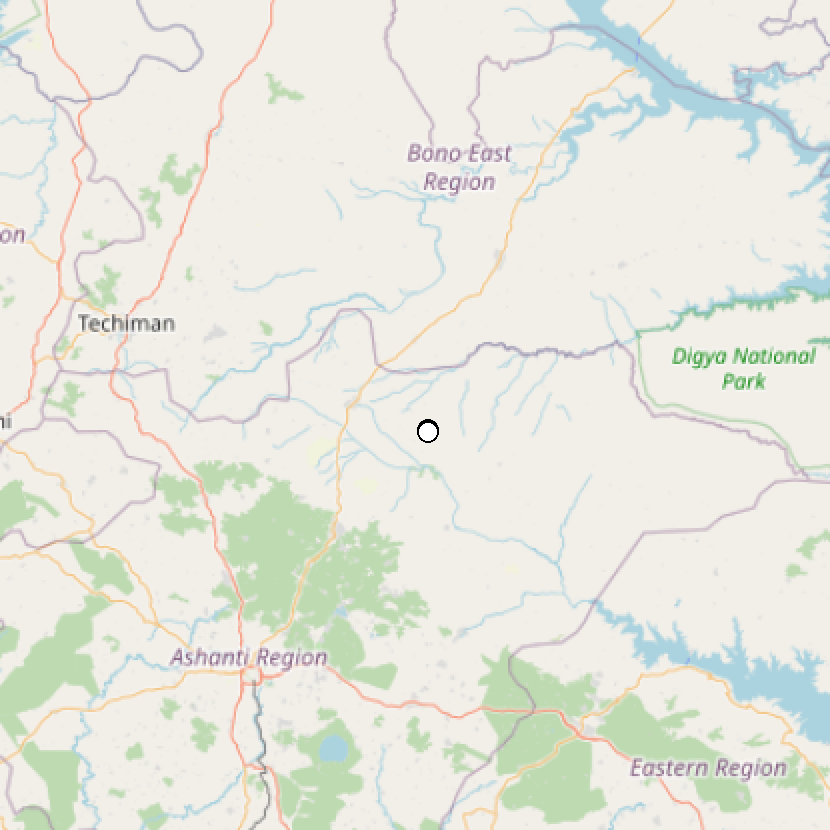
\includegraphics[width=4cm]{locationwide.png}
    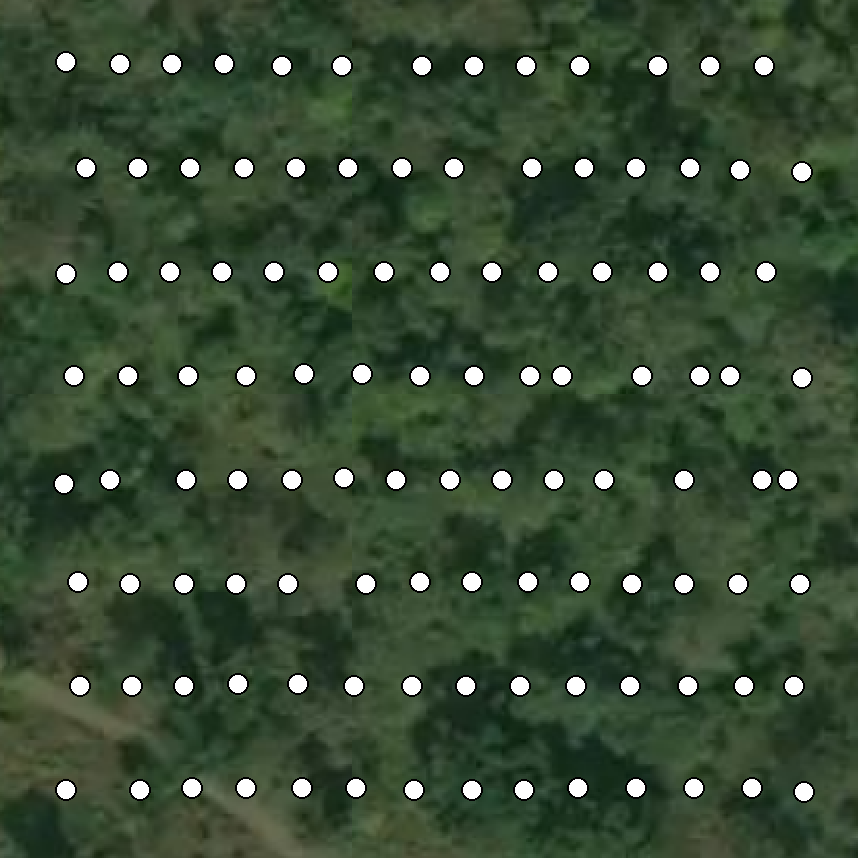
\includegraphics[width=4cm]{imgloc.png}
    \caption{Area of interest and unprocessed image GPS locations}
    \label{fig:areaofinterest}
\end{figure}


\subsection{Image Processing}
For image processing and DEM generation Agisoft Professional Edition 1.6.5 (Agisoft LLC., St. Peterburg, Russia) was used \citep{AgisoftMetashape}.
All data have been processed on the cloud service provided by Agisoft (\url{https://cloud.agisoft.com}).
The cloud processing is done on 32 vCPU's (Intel Xeon E5 2686 v4) with two NVIDIA Tesla M60 GPU's and 240 GB of RAM.

First, the complete data set has been aligned on medium quality.
On medium alignment quality, the original images are scaled to have 1/2 of the original size \citep{manual}.
Next, the dense cloud was built on medium quality (no depth filtering), resulting in a dense cloud of 3,268,264 points.
With medium settings, the original photo is scaled to 1/4 before used in the dense cloud generation process \citep{manual}.
A mesh was built using the triangulated irregular network (TIN) algorithm by \citet{axelsson1999processing}. 
Finally, after the mesh, the Reduce Overlap function was used to reduce the number of images used in the process of photogrammetry. 
Because the final product of the photogrammetry process in this paper is a DEM, a 2.5D height field was used when the mesh was generated.
The 2.5D height field mesh contains only one Z value for any X, Y coordinate combination, this is also the case in the final DEM.

\textbf{Reduce Overlap.} 
The algorithm of the Reduce Overlap function tries to select a minimal amount of images such that each point of the model is observed from N locations/angles.
If a point is observed multiple times from the same location/angle then this still counts as one observation. 
In this research a height field was used, the algorithm will take the vegetation canopy into account in the reconstruction, but lower branches may be lost in the process.
This will have some influence on the Reduce Overlap setting; it becomes more flexible because single height values are used for each X, Y coordinate combination.
The algorithm and parameters behind the Agisoft Reduce Overlap function are proprietary software and therefore unfortunately unknown.
In Agisoft Metashape the Reduce Overlap had three different settings: low, medium and high. 
All of the settings are used and the remaining images are used for further processing.
The images are matched based on an adapted version of the SIFT algorithm \citep{lowe1999object, AgisoftMetashape}.
All the datasets are processed on medium settings for image alignment.

\textbf{Dense Cloud.}
The alignment result of the images was used as input for the dense cloud generation.
The data were processed on medium settings without any depth filtering for the generation of the dense cloud. 
In Agisoft Metashape the dense cloud classification algorithm was used to classify the dense cloud in ground points and vegetation points. 
The vegetation was used as ground truth data for further analysis.

\textbf{DEM.}
The source data for the DEMs are the dense cloud results. 
The TIN algorithm was applied to build the DEMs \citep{axelsson1999processing}.
Because the dense clouds are unique, the TIN algorithm also results in four unique DEMs.
For further comparison, the DEMs have all been cropped on the largest common extent and the pixel resolution was set to 17.5 cm per pixel (1670 x 1290 pixels).
The DEMs were also scaled to check the differences between them without looking at the absolute values.
The scaling was done by subtracting the mean and dividing it by the standard deviation.
The scaled DEMs were subtracted from the scaled DEM that was created with all images.
This data was used to inspect the differences between the scaled DEM of the full image dataset compared to the other DEMs.

\section{Results}
In table \ref{tab:ImageProcessing} the image processing results can be found. 
It also contains the image processing results for the newly created datasets.
The lower the Reduce Overlap setting, the fewer images are left in a dataset and the fewer points are generated in the sparse cloud.
The dense clouds contain about the same amount of points except for the lowest Reduce Overlap setting.
The image set with the lowest image count has resulted in the dense cloud with the most points.

\begin{table}[h]
    \centering
    \caption{Reduce Overlap and Image Processing Results}
    \begin{tabular}{@{}cccc@{}}
    \toprule
    \textbf{\begin{tabular}[c]{@{}c@{}}Reduce Overlap \\ Setting\end{tabular}} &
    \textbf{\begin{tabular}[c]{@{}c@{}}Image\\ Count\end{tabular}} &
    \textbf{\begin{tabular}[c]{@{}c@{}}Sparse Cloud\\ Points\end{tabular}} &
    \textbf{\begin{tabular}[c]{@{}c@{}}Dense Cloud\\ Points\end{tabular}} \\ \midrule
    -      & 111 & 80,901 & 3,269,264 \\
    Low    & 44  & 37,886 & 4,172,783 \\
    Medium & 70  & 54,556 & 3,313,399 \\
    High   & 75  & 49,692 & 3,276,832 \\ \bottomrule
    \label{tab:ImageProcessing}
\end{tabular}
\end{table}

For all the different datasets the processing time can be found in table \ref{tab:processingTime}.  

\begin{table}[h]
    \centering
    \caption{Processing time in seconds for the difference steps in the process.}
    \label{tab:processingTime}
    \begin{tabular}{@{}cccc@{}}
    \toprule
    \textbf{Image Count} & \textbf{Sparse  Cloud} & \textbf{Dense Cloud} & \textbf{Dem} \\ \midrule
    111                  & 150                    & 292                  & 17           \\
    44                   & 59                     & 443                  & 16           \\
    70                   & 83                     & 147                  & 17           \\
    75                   & 129                    & 159                  & 17           \\ \bottomrule
    \end{tabular}
\end{table}

After all the new datasets with the images have been aligned, the camera locations are estimated.
In figure \ref{fig:cameralocation} camera locations can be found. 
None of the images used in the alignment process failed to align.


\begin{figure}[h]
    \centering
    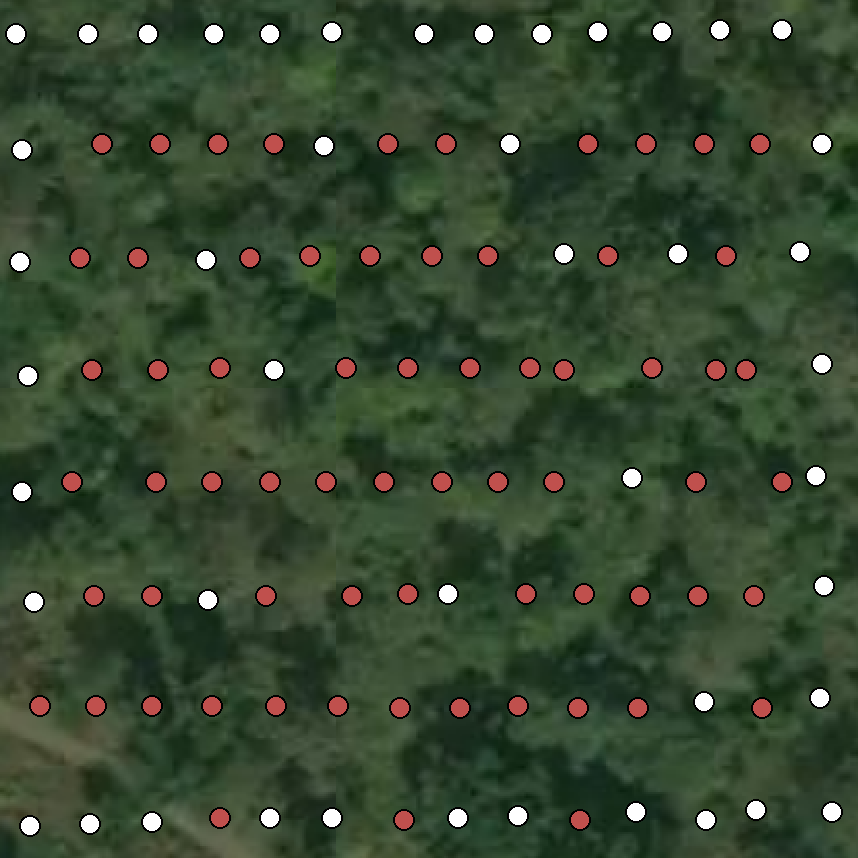
\includegraphics[width=1.9cm]{loc_low.png}
    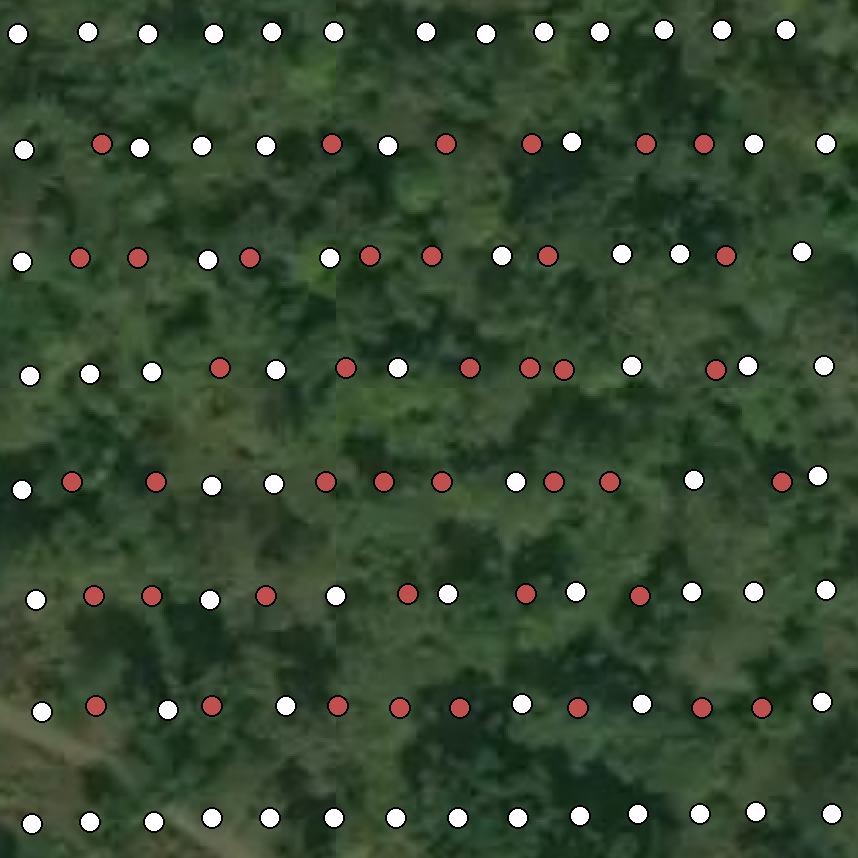
\includegraphics[width=1.9cm]{loc_med.png}
    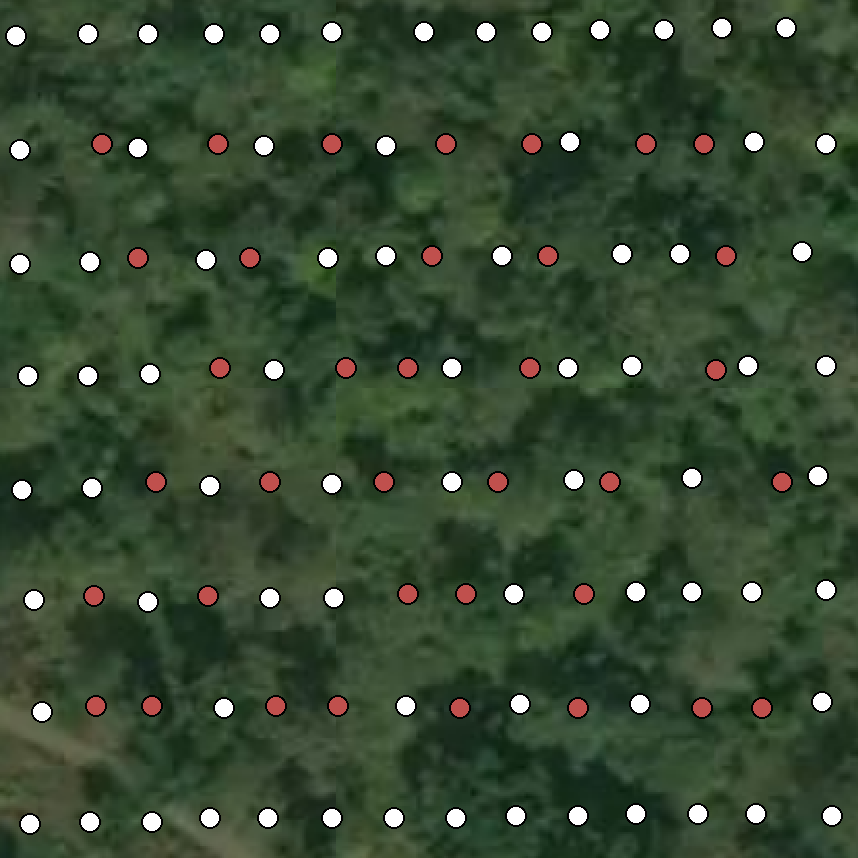
\includegraphics[width=1.9cm]{loc_high.png}
    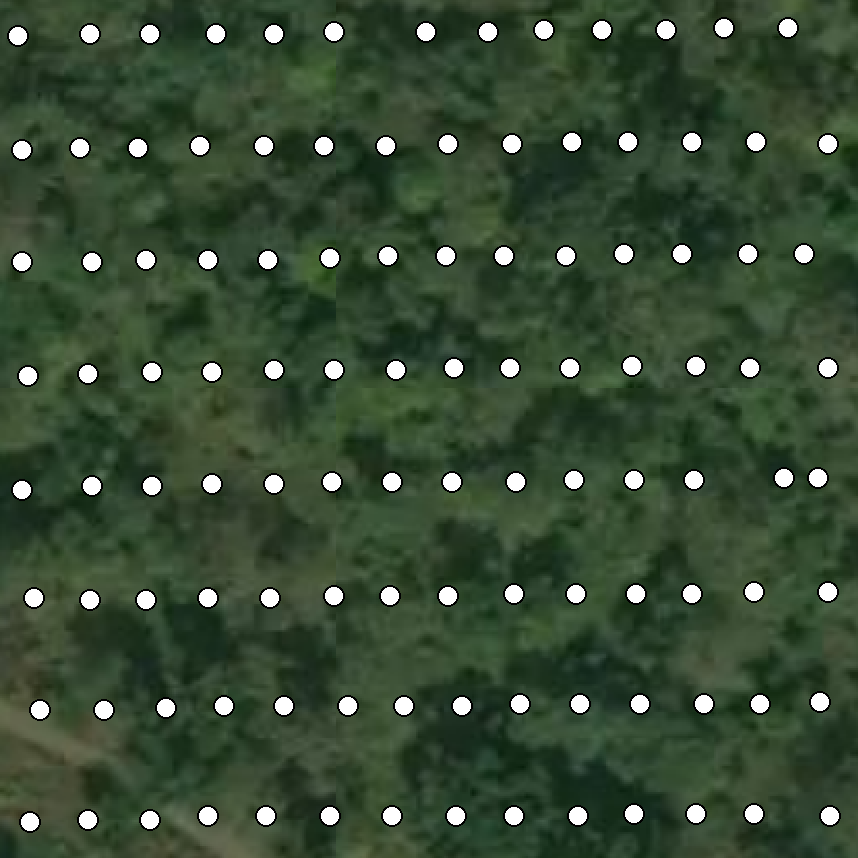
\includegraphics[width=1.9cm]{loc_full.png}
    \caption{Estimated camera location. 
    White: used in the image processing, red: disabled in the image processing.
    Starting left: low, medium, high and full settings}
    \label{fig:cameralocation}
\end{figure}

In figure \ref{fig:DemPlot_unscaled} the DEMs are visualized using the same colour range. 
The DEMs are distinguishable.

\begin{figure}[h!]
    \centering
    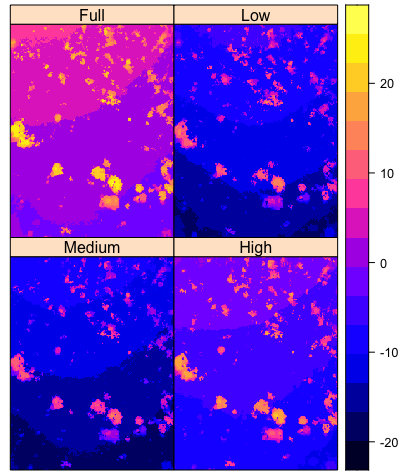
\includegraphics[width=6.5cm]{DEM2x2.png}
    \caption{DEM Results of the Reduce Overlap}
    \label{fig:DemPlot_unscaled}
\end{figure}

The boxplots in Figure \ref{fig:BoxPlot_unscaled} confirm this observation. 
For the low setting, the DEM values range from -19.4 to 19.0, for the medium setting the values range from -22.7 to 16.2, for the high setting the values range from 13.1 to 20.0 and for the full model from -4.8 to 28.9. 
Units are in meters.

\begin{figure}[h!]
    \centering
    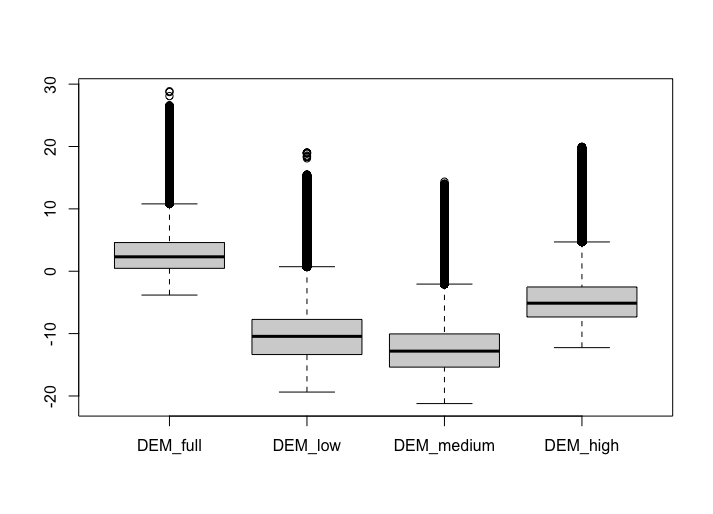
\includegraphics[width=7.5cm]{DemBoxplot.png}
    \caption{Box plots of the DEM results of the Reduce Overlap}
    \label{fig:BoxPlot_unscaled}
\end{figure}

Figure \ref{fig:DemPlot_scaled} contains the same visualization of DEM plots, only for all the DEMs, the data has been scaled.
The DEMs look similar in this figure.

\begin{figure}[h]
    \centering
    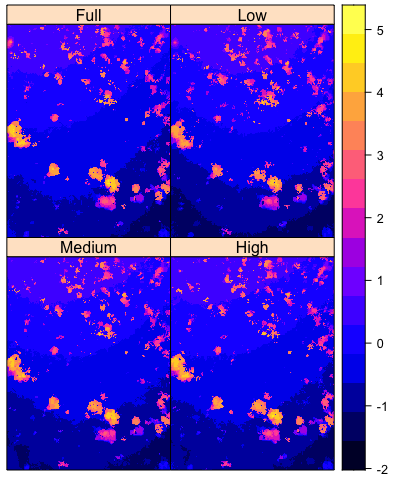
\includegraphics[width=6.5cm]{DEM2x2_scaled.png}
    \caption{Scaled DEM Results of the Reduce Overlap}
    \label{fig:DemPlot_scaled}
\end{figure}

This is confirmed in figure \ref{fig:BoxPlot_scaled}, only now the boxplot contain the scaled data values.
The differences seem to be minimal in the scaled boxplots.

\begin{figure}[h!]
    \centering
    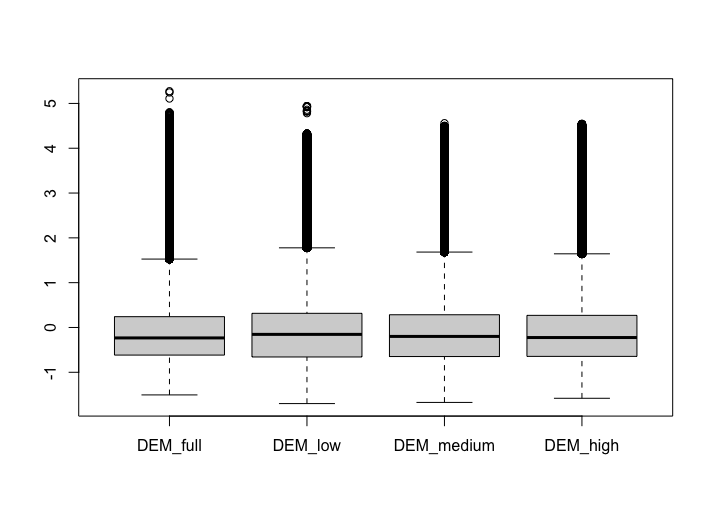
\includegraphics[width=7.5cm]{DemBoxPlot_Scaled.png}
    \caption{Scaled DEM Results of the Reduce Overlap}
    \label{fig:BoxPlot_scaled}
\end{figure}

Figure \ref{fig:ViolinPlot} contains three violin plots. 
For each of the plots, the scaled DEMs from the reduced image datasets has been subtracted from the scaled full dataset DEM.
It is visible that the overall scaled error difference of the scaled DEMs varies from around -5.0 to 5.0.
For the high settings, the differences are more centered around zero, while this is not the case for low and medium settings.
For the medium setting, the difference is slightly more centered around 0.0 than in the low setting.

\begin{figure}[h]
    \centering
    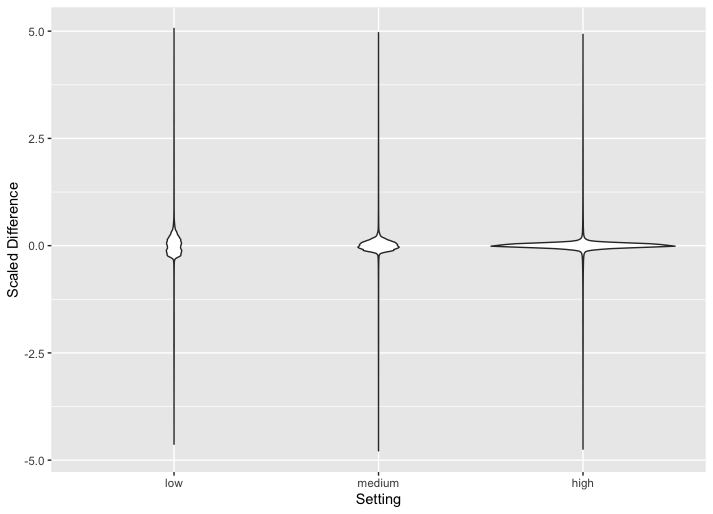
\includegraphics[width=6.5cm]{ViolinPlotOrdered.png}
    \caption{Violin plot of the difference between the full DEM and the reduced DEMs. All violin plots contain 2.154.300 measurements (1.670 rows x 1.290 columns)}
    \label{fig:ViolinPlot}
\end{figure}

In figure \ref{fig:ScaledDifference} the differences of the scaled DEMs have been plotted on top of the ground truth vegetation.

\begin{figure}[h]
    \centering
    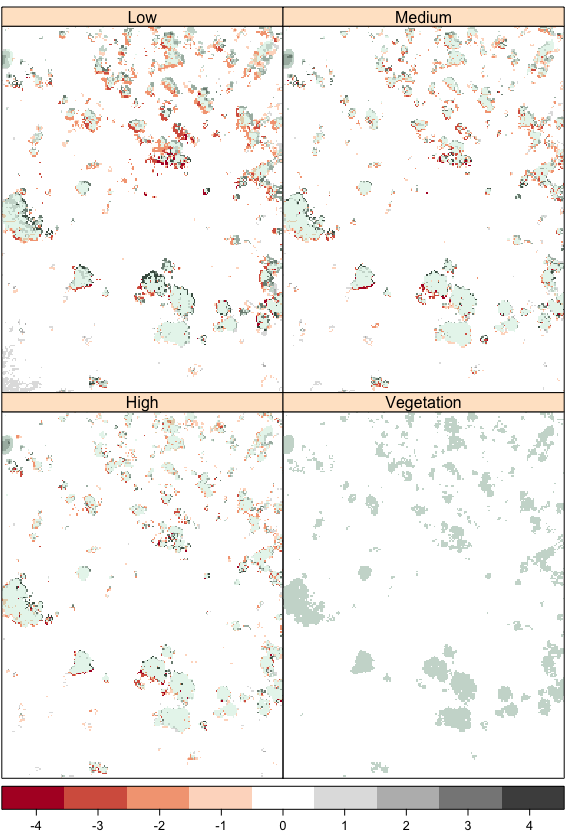
\includegraphics[width=7cm]{finalvegplot.png}
    \caption{The difference between the original DEM and the scaled DEMs from the reduced image datasets. Negative differences are red and positive differences are grey. The vegetation ground truth data has been plotted in the right bottom with a light green color and underneath the differences.}
    \label{fig:ScaledDifference}
\end{figure}

\section{Discussion}
The goal of this research was to see how a different image overlap of the same areas influences the different steps in the photogrammetry pipeline and especially the DEM result.
The processing time is also investigated.
The image reduction in the paper was done in Agisoft Metashape with the Reduce Overlap function.

The processing time and the alignment of the images are dependent on the image count.
Fewer images result in less computation time, but also fewer points in the sparse cloud.
The amount of images used in the processing does not seem to influence the density of the dense cloud, which was also concluded by \citet{EffectofUABimgcamover}. 
The only exception was building the dense cloud for the image data set with the lowest count. 
The lowest image count resulted in the dense cloud with the highest point count.
Because of this, the processing time for this dense cloud was higher compared to the other datasets.
However, the image count does influence the time needed to generate the dense cloud; more images means more time needed.
There is no time difference in the generation of the DEMs.
It is not a computationally expensive step and therefore no differences can be detected.

There is a large difference between the absolute values of the different DEMs, this can be seen visually in figure \ref{fig:DemPlot_unscaled} and also when comparing the boxplot values in figure \ref{fig:BoxPlot_unscaled}.
The outliers in both boxplot figures are probably the vegetation that is present in the area as the boxplots only contain high outliers.
With the use of at least three ground control points, the error in the dense cloud will be reduced \citep{AssessingUAVGCPS, GCPbetterAccuracy, GeoreferencedPointClouds}.
As the relative points in all of the DEMs do not differ, using ground control points can correct the absolute error value.
In the end, this will result in a dense cloud with a higher point accuracy and fewer errors in the absolute values of the DEM.

The violin plots indicate that the dataset with the highest image count is most similar to the full dataset. 
The difference of the scaled DEMs is more centered around zero, while the two lower image count datasets are more widespread.
The largest errors differences (around -5/5) between the scaled DEM seem to be the same for all the image datasets.
This is confirmed by looking at the difference between the scaled DEMs in \ref{fig:ScaledDifference}.
Agisoft Metashape seems to have difficulties in modelling the complex structures of the vegetation with less image overlap, which is visually confirmed in figure \ref{fig:ScaledDifference}. 
In this figure larger errors are visible around the vegetation.
\citet{AccessingImageOverlap} also concluded that a high image overlap is needed to model complex structures.
Another option could be changing the filtering setting provided by the Metashape dense cloud generation.
In this research, no depth filtering was used.
By applying a more aggressive filtering algorithm the complex structures of the vegetation will be lost in the DEM generation and therefore will not appear as errors anymore in the comparison \citep{AgisoftMetashape}.
If the final product from the photogrammetry pipeline is a DEM, a lower image overlap can be used as most of the differences compared to the full image dataset appear around the vegetation and not in the ground elevation.

\section{Conclusion}
The image overlap does influence the processing time in the photogrammetry process. 
More images mean more processing time.
Using different image overlap of the same area results in DEMs with different absolute values.
The two image datasets with the least images show the largest difference in absolute value range compared to the original dataset with all images.
The image dataset with the highest image count has a DEM that is most similar compared to the original dataset.
When the scaled values are compared, there seems to be a minimal difference between the DEMs.
If more images are used in the dataset, the difference between the scaled DEMs becomes smaller.
The differences all seem to occur around the vegetation.


% KAO: Sloppy spacing ensures non-overfull lines. Can be removed if this is not an issue.
\sloppy




{
	\begin{spacing}{1.17}
		\normalsize
		\bibliography{bibliography} % Include your own bibliography (*.bib), style is given in isprs.cls
	\end{spacing}
}



\vspace{1cm}
\end{document}



